% Created 2018-05-13 Sun 14:09
\documentclass[a4paper,11pt]{article}
                % input
                \usepackage[utf8]{luainputenc}
                \usepackage{fontspec}
                \usepackage{unicode-math}
                \usepackage[novoc]{arabluatex}
                \newfontfamily\arabicfont[Script=Arabic]{Scheherazade}
                \newcommand{\arbt}[1]{\Large{\arb{#1}}} %{\arbt{...}}
                \newcommand{\arbT}[1]{\LARGE\arb{#1}} %\arbT{...}
                % layout
                \usepackage{layout}
                \usepackage{setspace} %package pour les interlignes
                \usepackage{multicol}
                \setlength{\columnsep}{40pt}
                \usepackage{xcolor} % package pour les couleurs
                % headers ...
                \usepackage{fancyhdr} % header etc
                \usepackage{fancybox} %package pour les encadrements supp
                \pagestyle{fancy} % Use en-tetes et des pieds de page personnaliser grâce fancyhdr
                \usepackage[Glenn]{fncychap}
                \fancyhead[L, R, C]{} % définition en-tête
                \fancyfoot[L, R]{} % définition pied de page
                \fancyfoot[C]{\thepage}
           		\renewcommand{\headrulewidth}{0pt} % ligne haut out
	        	\renewcommand{\footrulewidth}{0pt} % ligne bas out
                % others
                \usepackage{float}
                \usepackage{array, makecell} %pour les tableaux et makecell pour les cellules
                \usepackage{multirow} %pr tableau
                \newcolumntype{P}[1]{>{\centering\arraybackslash}m{#1}} %P{taille}
                % maths
                \usepackage{amsmath, amsthm} %package pour les maths
                \usepackage{lettrine}
                \usepackage{marvosym} %package de symbole
                % others
                \usepackage{wrapfig} % pour les capsules in text
                %defaut emacs packages
                \usepackage{fixltx2e}
                \usepackage{graphicx}
                \usepackage{longtable}
                \usepackage{float}
                \usepackage{wrapfig}
                \usepackage{rotating}
                \usepackage[normalem]{ulem}
                \usepackage{textcomp}
                \usepackage{wasysym}
                \usepackage{hyperref}
               

\usepackage[top=2cm, bottom=2cm, left=2cm, right=2cm]{geometry}
\author{Gueye Ousseynou\thanks{21505055.}}
\date{\today}
\title{\textbf{Documentation devoir sur FCA} \\ Cours de logique - S6}
\hypersetup{
  pdfkeywords={},
  pdfsubject={...},
  pdfcreator={...}}
\begin{document}

\maketitle
\setcounter{tocdepth}{3}
\tableofcontents

\section{Sujet}
\label{sec-1}

Réaliser une analyse formelle de concepts sur la NBA, ligue de basketball américaine. \\

\section{Concepts utilisés}
\label{sec-2}

\begin{itemize}
\item \textbf{conf\_est} : Pour des raisons géographiques, la NBA division les équipes en deux conférences est et ouest. Chaque équipe est soit dans l'une, soit dans l'autre. \\

\item \textbf{playoffs\_2018} : la NBA est active entre octobre et juin. La saison est divisée en deux partie : une \textbf{saison régulière}, où chaque équipe (32) joue un total de 82 matchs. À l'issue de la saison réguliére, les 16 meilleures équipe s'affrontent dans ce que l'on appelle les \textbf{playoffs}. Chaque couple d'équipes s'affronte au meilleur de 7 matchs, le vainqueur accédant au niveau suivant. \\
\end{itemize}

Nous avons : le 1er tour, les demi-finales de conférences, les finales de conférences et la grande finale. \\

Dans cette colonne, on regarde les équipes qualifiées pour les playoffs de cette année 2017-2018. \\

\begin{itemize}
\item \textbf{mvp\_10} : à l'issue de la saisons régulières dont nous avons parlé, on élit le MVP pour most valuable player. C'est probablement la plus haute distinction, à part celle de gagner le titre. \\
\end{itemize}

Dans cette colonne, on regarde les équipes dont un des joueurs fut MVP au cours des 10 dernières années. \\

\begin{itemize}
\item \textbf{titre\_10} : dans cette colonne, on regarde les équipes ayant gagné le titre au cours des 10 dernières années. \\

\item \textbf{contenders} : Simple prédiction, j'ai considéré les équipes me paraissant pouvoir concourir pour gagner le titre. C'était il y a un mois, donc juste au début des playoffs. \\
\end{itemize}

\section{Résultats et interprétation}
\label{sec-3}

Voici le rendu, que nous avons modifié pour faire apparaitre ce que nous avons trouvé intéressant \\

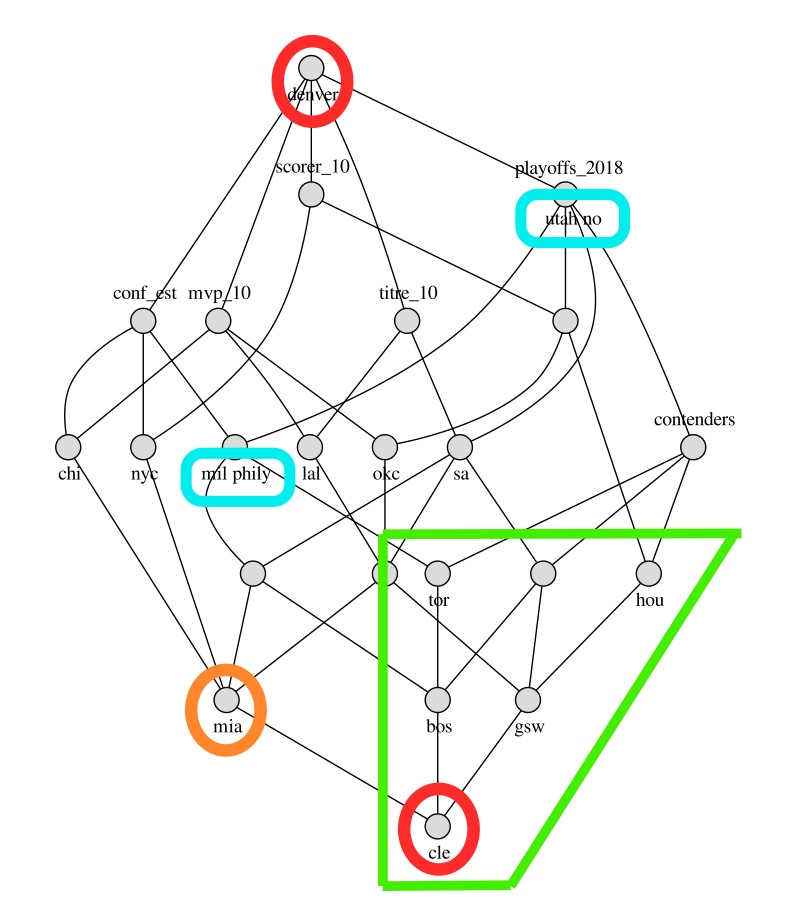
\includegraphics[width=.9\linewidth]{./img/rendu_annote.jpg} \\

\subsection{Interprétation}
\label{sec-3-1}

\begin{itemize}
\item \textbf{En rouge} : nous avons deux équipes : Cleveland et Denver, placées aux deux sommets de notre image. \\
\end{itemize}

Pour faire simple, Cleveland est proche de ce que la NBA peut donner de meilleur, aussi bien en terme de résultats collectifs que de récompenses individuelles. \\

De l'autre côté, Denver est ce qu'il y a de pire. En plus de 10 ans où je suis la NBA, je n'ai jamais vu denver gagné la moindre petite chose. \\

Cependant, il est intéressant de noter que la réussite de Cleveland, tient à un seul homme : Lebron James. \\

Paraphrasant Lamartine, je dirais que parfois il suffit d'un seul joueur pour que tout vous réussisse. \\

\begin{itemize}
\item \textbf{En bleu} : ce sont les seuls points que deux équipes partagent : d'un côté (Utah et New Orleans), de l'autre (Milwaukee et Philadelphia). Le regroupement est d'abord dû à la conférence. \\
\end{itemize}

Ces 4 équipes sont en playoffs, mais trop jeunes, elles n'espéraient pas gagner le titre. Par contre, chacune d´elle peut représenter le futur de sa conférence. Ainsi, si nous refaisons le même tableau dans quelques années, je pense que de chaque couple ne restera qu'une équipe. \\

\begin{itemize}
\item \textbf{En orange} : nous avons une équipe (Miami) qui malgré des résultats modestes cette année est bien placée. C'est surtout du à son passé. Et la passage d'un homme : Lebron James qui y a joué de 2010 à 2014. \\

\item \textbf{En vert} : Nous avons 5 équipes : Toronto, Houston, Boston, Golden State et Cleveland. \\
\end{itemize}

N'oublions pas que le concept "contenders" était basé sur nos prévisions. Un mois plus tard, nous sommes aux finales de conférences, donc il ne reste que 4 équipes en compétitions. Et il se trouve que les 4 équipes les plus à droite sont celles restantes. La seule éliminée est Toronto. \\

Le pari fut donc gagnant. \\
% ...
\end{document}